\subsection{Additional Details in Reproducing DAPO Training}
\label{supp_sec:dapo_repro}

Our reproduction was conducted on 32 AMD MI300X GPUs using the VERL framework~\citep{sheng2025VERL}, and ran for over two weeks.
Our run did not fully reproduce the $Pass@1$ accuracy above 50\% as reported by~\citet{yu2025DAPO-Zero}, while we reached a comparable performance of around 44\% $Pass@1$, in line with a third-party reproduction~\citep{chen2025NFT}.
We use the same verifier introduced in Section~\ref{sec:benchmark_analysis} to assess the correctness of both training and evaluation rollouts.

\begin{figure*}[t]
  \centering
    \subfigure[
    Distributions of $P(CA)^{(q)}$ and $P(CC|CA)^{(q)}$ for \textbf{easy} training questions in DAPO.
    ]{
    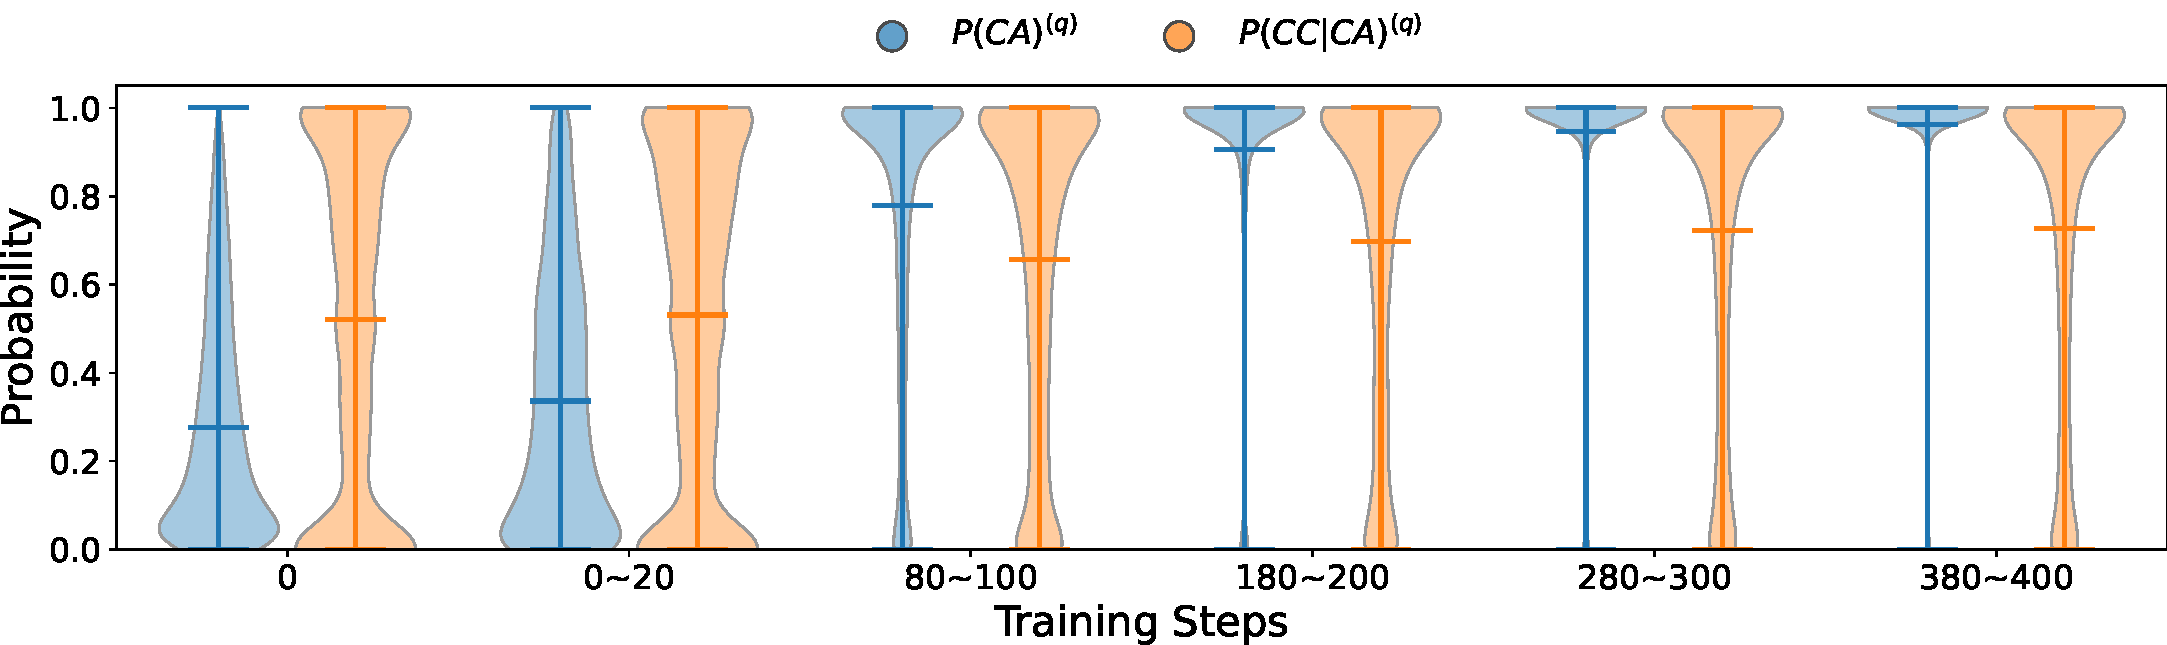
\includegraphics[width=0.95\linewidth]{figures/rollout_verify_easy.pdf}
    \label{fig:easy_q_ca_cc_in_training}
    } \\
    \vspace{-5pt}
    \subfigure[
    Distributions of $P(CA)^{(q)}$ and $P(CC|CA)^{(q)}$ for \textbf{hard} training questions in DAPO.
    ]{
    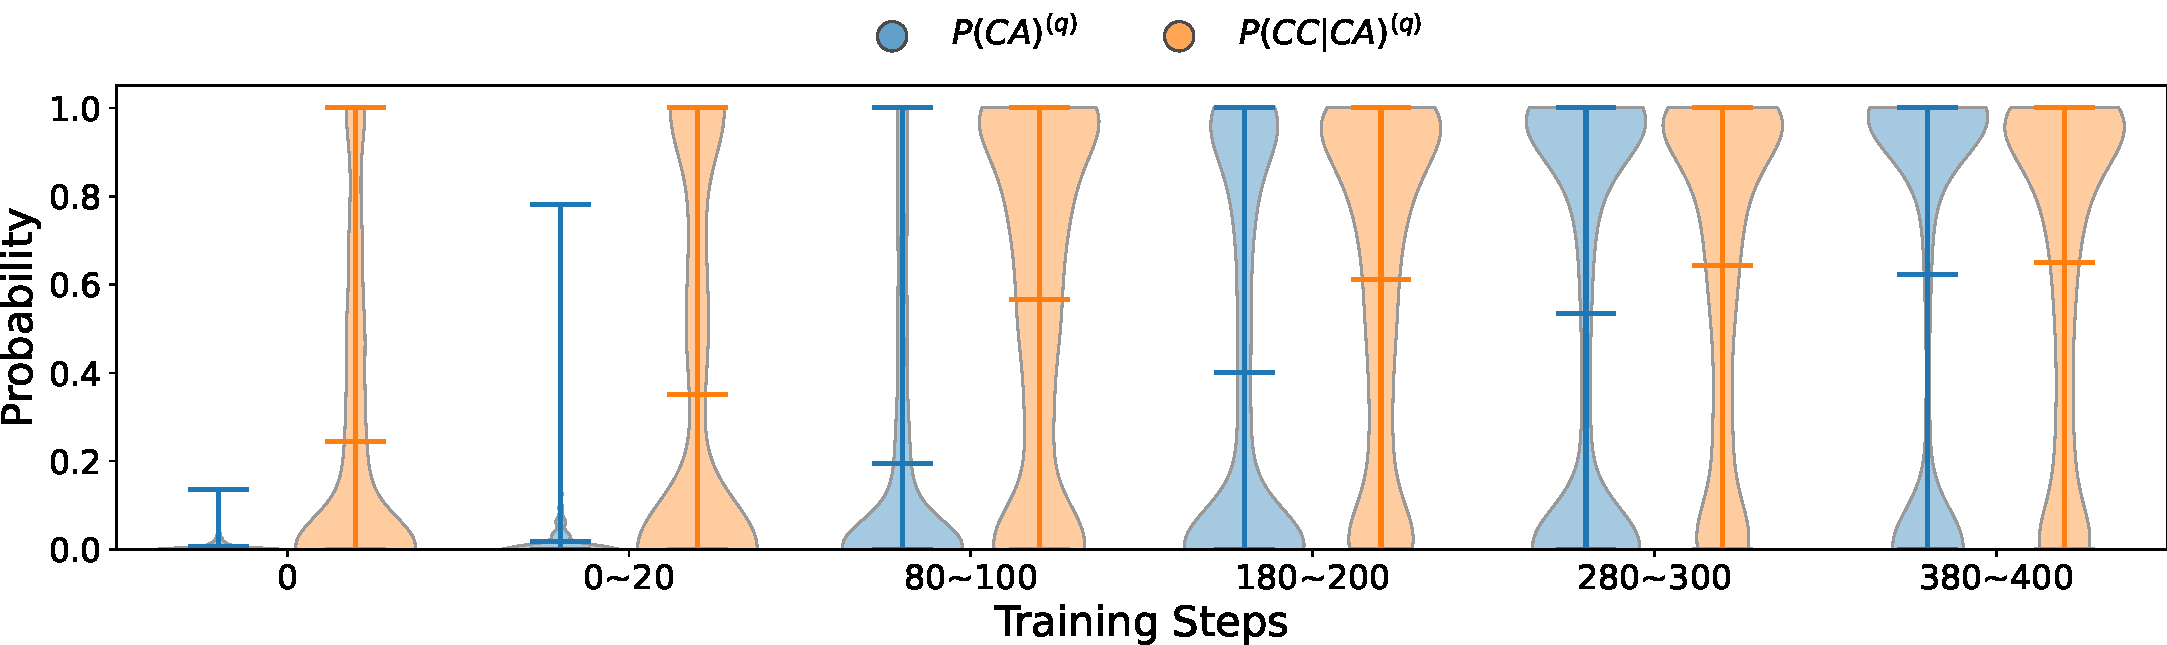
\includegraphics[width=0.95\linewidth]{figures/rollout_verify_hard.pdf}
    \label{fig:hard_q_ca_cc_in_training}
    } \\
    \vspace{-5pt}
    \subfigure[
    Generalization performance on AIME 2024 across different training steps.
    ]{
    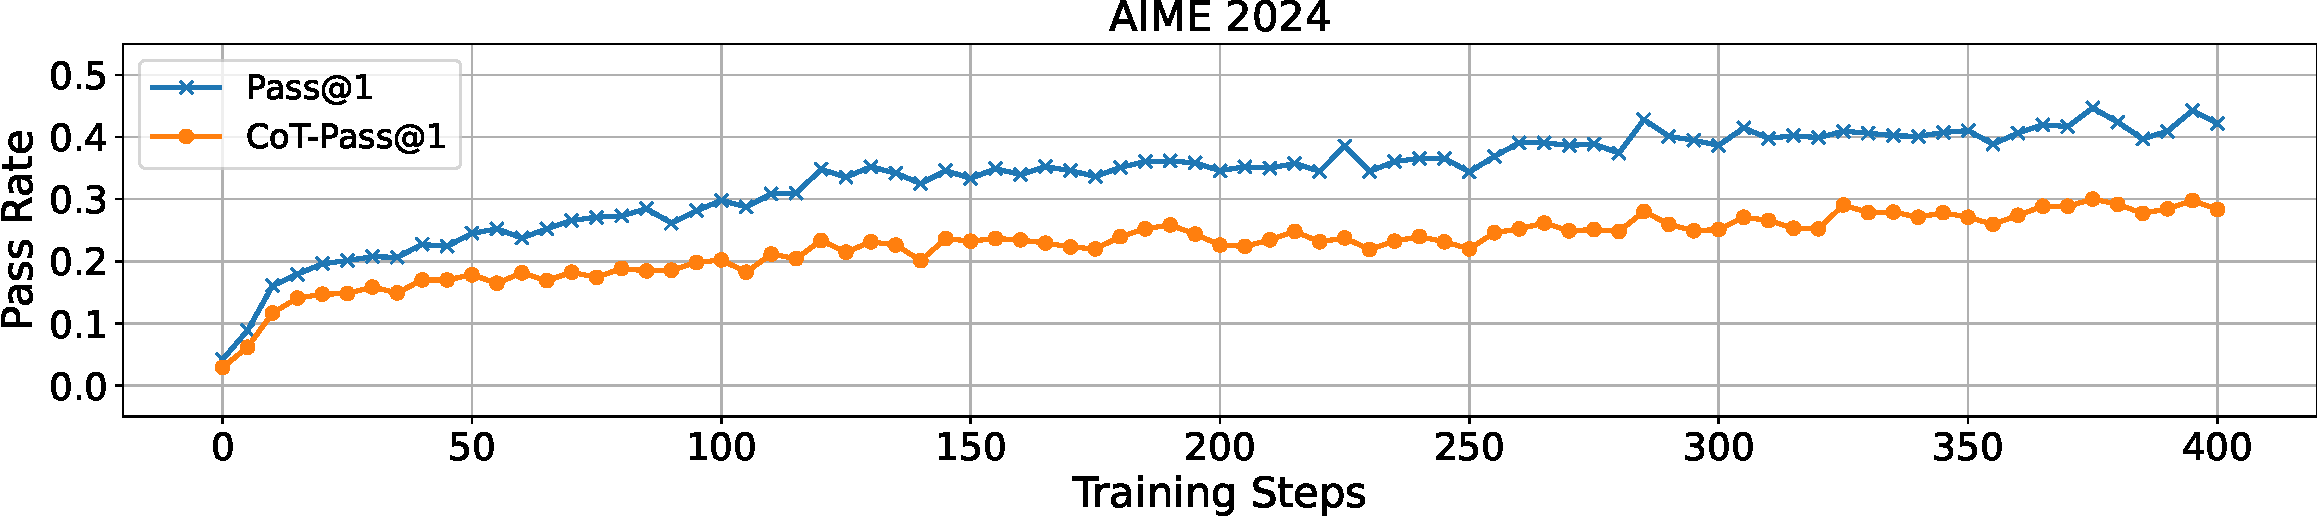
\includegraphics[width=0.95\textwidth]{figures/dapo_process_val_pass1.pdf}
    \label{fig:aime24_val_in_training}
    }
\caption{
We show gradually optimized performance on training prompts throughout RLVR and corresponding generalization behaviors on testing prompts.
The top two subfigures use violin plots to visualize the evolution of $P(CA)^{(q)}$ (the fraction of correct answers for prompt $q$) and $P(CC|CA)^{(q)}$ (the fraction of correct CoTs within the correct answers for prompt $q$) over the course of DAPO training.
Subfigure (a) shows results for ``easy'' training questions, while (b) presents the corresponding distributions for ``hard'' questions ($P(CA)^{(q)}$ < 1 for DAPO).
We divide training questions into easy and hard by sampling 64 rollouts for each of the $17k$ training questions using Qwen2.5-32B, and labeling those with at least one correct answer as easy.
Subfigure (c) presents the generalization performance on AIME 2024 across different training steps.
}
\label{fig:dapo_training_analysis_supp}
\end{figure*}

In addition to the performance evolution on fully optimized training questions highlighted in Figure~\ref{fig:q_ca_cc_in_training} of the main paper, we include performance evolution on hard questions and more continuous validation performance in Figure~\ref{fig:dapo_training_analysis_supp} to provide more comprehensive information.
The additional observations are consistent with what we have introduced in the main paper.
It is natural to observe that RLVR begins to incentivize correct reasoning from the very beginning, as evidenced by increased $P(CC|CA)^{(q)}$ values in the early training steps shown in Figures~\ref{fig:easy_q_ca_cc_in_training} and~\ref{fig:hard_q_ca_cc_in_training}.
These incentivized reasoning capabilities translate into improved generalization on unseen questions, as demonstrated by notable gains in CoT-Pass@K on AIME 2024 within the first 20 training steps in Figure~\ref{fig:aime24_val_in_training}.
Note that each training step here corresponds to one round of PPO-style optimization~\citep{schulman2017PPO}, which includes 16 gradient updates, according to the DAPO training script.
Thus, we see that correct reasoning abilities begin to generalize after only a few gradient updates.

Furthermore, the incentivization of correct reasoning on training questions appears to be a continuous process, as reflected by the steady increase in the mean of $P(CC|CA)^{(q)}$ throughout training, for both easy and hard questions.
Meanwhile, we again observe that $P(CA)^{(q)}$ (equivalent to $Pass@1^{(q)}$) is an unreliable metric, particularly for easy training questions.
As shown in Figure~\ref{fig:easy_q_ca_cc_in_training}, the distribution of $P(CA)^{(q)}$ becomes highly skewed toward $1.0$ after 180 steps, misleadingly suggesting that most questions are perfectly solved.
However, examining the distribution of $P(CC|CA)^{(q)}$ reveals that a substantial fraction of responses still contain flawed reasoning.
We suspect this is one of the reasons behind the difficulty of achieving strong results with Qwen2.5-32B using the R1-zero approach.

For both easy and hard training questions, improving $P(CC|CA)^{(q)}$ seems to be a slow and challenging process. Since our analysis shows that enhancing correct CoTs is key to improving reasoning capabilities, we believe that future research should explore novel mechanisms to accelerate the improvement of $P(CC|CA)^{(q)}$, thereby enhancing both the efficiency and effectiveness of RLVR.
